\section{Data Collection}\label{sec:data}

Home routers can observe many aspects of home networks because typically all
other devices in the home communicate both to each other and to the Internet via
the router. Over the past three years, we have deployed routers in 126 homes across
19 countries. Each router measures the quality of the upstream Internet
connection and collects limited information about device usage on the home
network. This section introduces the router platform, the data we collect from
the routers, and that data's implications for our study.

\begin{figure}[t!]
 \begin{center}
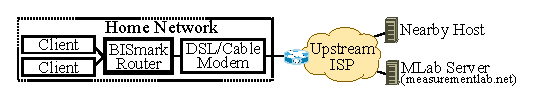
\includegraphics{figures/schematic-cacm.eps}
\caption{The BISmark home router sits directly behind
  the modem in the home network.  It collects both active and passive
  measurements.}\label{fig:bismark-deployment} 
\end{center}
\end{figure}


%\vfill
\subsection{Collection Infrastructure}

\name{} comprises gateways in the home, a centralized management and
data collection server, and several measurement servers. We have
instrumented the gateway with custom firmware that performs both passive
and active measurements. Where appropriate, the firmware anonymizes
certain aspects of the data before sending them back to the central
repository for further analysis.  Figure~\ref{fig:bismark-deployment}
shows a typical deployment in the home network, and how BISmark performs
its measurements.

\paragraph{Firmware.} \name{} is a custom home router firmware based on OpenWrt
for Netgear WNDR3800 and WNDR3700v2 routers~\cite{www-openwrt,www-netgear-3800}.
Routers have a 450~MHz MIPs processor, 16~MB of flash storage, 64~MB of RAM, an
Atheros wireless chipset, one 802.11gn radio, and one 802.11an radio.
\name{} typically replaces a household's wireless access point and connects
directly to the cable or DSL modem that provides Internet access to that
household. Because the router sits on the path between the user's home network
and the rest of the Internet, our software is uniquely positioned to capture
information about both the characteristics of network connectivity and of home
network usage (\eg, usage patterns, applications). We expected routers to remain
powered on almost all the time, since they provide the household's Internet
connectivity; however, later in this paper we show that this assumption does not
hold in several countries and regions.

\paragraph{Recruiting and deployment.} Our deployment of routers across
home networks has been organic: We have recruited most of our users by
word-of-mouth, or through targeted advertisements for specific
experiments and projects that we have run as part of our research.  For
example, the router firmware performs continuous measurements of the
performance of the home access link, which has garnered the attention of
various policy and regulatory agencies.  We have also performed smaller
recruitment efforts in various areas for a usage cap management tool
that we built on top of the firmware~\cite{kim2011communicating}.
Depending on the experiments that different users have consented to (or
not), we are able to collect different types of information.  Most users
have remained actively engaged in our experiments by virtue of the fact
that they receive a free router as a result of their participation.

%We classify the countries where we have deployed routers into two groups
%based on the GDP (Gross Domestic Product) per capita ranking in year
%2011~\cite{www-gdp}.  We call countries for whom the per capita GDP
%falls within the top 50 \groupa{}; in our deployment, these countries
%were: Switzerland, Spain, United States, Italy, Japan, Canada,
%Netherlands, Germany, Singapore, Israel, United Kingdom, Hong Kong, and
%France.  Otherwise, we define them as \groupb{}; countries in our
%deployment in this group were: India, Pakistan, Malaysia, South Africa,
%Mexico, China, Brazil, Indonesia.
We classify the countries where we have deployed routers into two groups based
on the GDP (Gross Domestic Product) per capita ranking in year
2011~\cite{www-gdp}.  We call countries for whom the per capita GDP falls
within the top 50 {\em \developed{}}; otherwise, we call them {\em \developing{}}. Table~\ref{tab:grouping}
summarizes this grouping.
%Note that we use {\em developed
%countries} for \groupa{} and {\em developing countries} for \groupb{}
%interchangeably throughout the paper.

\begin{figure}[t!]
 \begin{center}
 \frame{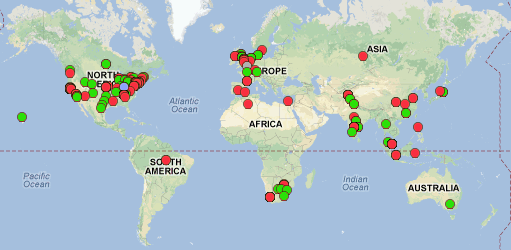
\includegraphics[width=\linewidth]{figures/bismark-may2013}}
\caption{The BISmark deployment as of May 2013.  Each dot indicates a
  router.  The green dots indicate routers that are currently
  reporting~(156).  Because we only use data from routers that
  consistently report data throughout the period of our study, we use
  data from 126 routers in 19 countries.  The red dots include the
  full set of routers that have ever contributed
  data~(295).}\label{fig:bismark-deployment-map}
\end{center}
\end{figure}


%%
%\begin{table}[t]
%\small
%\begin{tabular}{m{0.14\columnwidth}|m{0.60\columnwidth}|m{0.12\columnwidth}}
%{\bf Group} & {\bf Countries} & {\bf Total Routers}\\
%\hline
%{\developed{}} & {Canada, Germany, France, United Kingdom, Ireland, Italy, Japan, Netherlands,  Singapore, United States} & {90}\\
%\hline
%{\developing{}} & {India, Pakistan, Malaysia, South Africa, Mexico, China, Brazil, Indonesia, Thailand} & {36}\\
%\end{tabular}
%\centering\caption{Classification of countries based on GDP per capita.}
%\label{tab:grouping}
%\end{table}
\begin{table}[t]
\small
\begin{tabular}{m{0.30\columnwidth} m{0.10\columnwidth} | m{0.30\columnwidth} m{0.10\columnwidth}}
{\bf Developed} & {\bf Routers} & {\bf Developing} & {\bf Routers}\\
\hline
Canada & 2 & India & 12\\
Germany & 2 & Pakistan & 5\\
France & 1 & Malaysia & 1\\
United Kingdom & 12 & South Africa & 10\\
Ireland & 2 & Mexico & 2\\
Italy & 1 & China & 2\\
Japan & 2 & Brazil & 2\\
Netherlands & 3 & Indonesia & 1\\
Singapore & 2 & Thailand & 1\\
United States & 63 & {} & {}\\
\hline
Total Routers & 90 & Total Routers  & 36\\
\end{tabular}
\centering\caption{Classification of countries based on GDP per capita.}
\label{tab:grouping}
\end{table}
%%

\subsection{Data}

\begin{table}[t]
    \small
    \begin{tabular}{l|r|r|r}
        Dataset & Routers & Countries & Dates \\
        \hline
        \multicolumn{4}{c}{{\em Active measurements}} \\ \hline
        Heartbeats & 126 & 19 & October 1, 2012--April 15, 2013 \\
        Capacity & 126 & 19 & April 1--April 15, 2013 \\ \hline
        \multicolumn{4}{c}{{\em Passive measurements}} \\ \hline
        Uptime & 113 & 19 & March 6--April 15, 2013 \\
        Devices & 113 & 19 & March 6--April 15, 2013 \\ %April ?
        WiFi & 93 & 15 & Nov. 1--Nov. 15, 2012 \\
        Traffic & 25 & 1 & April 1--April 15, 2013 \\
    \end{tabular}
    \caption{Summary of data collected for this study.  With the
      exception of the Traffic data set, which is subject to privacy
    restrictions, we will publicly release all data used in this study.}
    \label{table:datasets}
\end{table}

We now summarize the data we collected from the BISmark deployment, then
describe each data set in more detail.  We will also highlight some
factors that limit the conclusions we can (or cannot) draw from our
data.  Where possible, we have released the data collected from this
study; the Capacity data (described below) is publicly available and is
also continuously updated as the routers collect new
measurements.\footnote{\url{http://uploads.projectbismark.net}} We have
released all measurements that do not have personally identifying
information (PII) (\ie, everything except the Traffic data
set).\footnote{\url{http://data.gtnoise.net/bismark/imc2013/nat}}

\subsubsection{Summary}

Table~\ref{table:datasets} summarizes the data we collected from our deployment.
\name{} routers perform both active and passive measurements. Many routers only
collect performance measurements about the router's upstream Internet connection
and basic diagnostic information about the number of connected devices; these
measurements record no personally identifying information (PII) and, as a
result, do not require written consent. In twenty-five homes
where we have explicit consent, we collect additional information about the
activity of users and devices on the home network; for those households we
clearly explained the risks of PII exposure and obtained written
consent.\footnote{Our university's Institutional Review Board (IRB) certified
all aspects of our data collection and experiments.} Engineering and consent
constraints dictated that we collect the data sets over different time periods.
We now explain each data set in more detail.

%TODO Explain anonymization procedures
% bismark-passive
%   - Overview of data collected
%   - Deployed on total of 42 routers, 34 have significant data
%   - Although we collected data for over a year, we concentrate on October
%   2012, when there were 23 active devices (21 without significant outages.)
%  - UPDATE: April 1 - 14 has 28 active devices (removing 3 since they are <100mb = 25 considered).
% bismark-active
% bismark-health
%   - uptime
%   - ethernet ports
% bdm pings

\subsubsection{Measurements}

\paragraph{Heartbeats.} Every router sends a ``heartbeat'' packet to the central
\name{} server approximately once a minute. We use this data to measure router
uptime. A heartbeat packet indicates that the router is on and online,
but a lost packet could mean a router is powered off, offline, or has
lossy connectivity to the server.  These heartbeats can be lost, and the
router makes no attempt to retransmit them. They are
nonetheless frequent enough to provide reasonable confidence
about the uptime of each \name{} router, which we analyze in
Section~\ref{sec:availability}. We consider heartbeats from 126 routers
that were on for at least 25 days between October 2012 and April 2013.

\paragraph{Uptime.} Starting in March of 2013, each router sends its uptime
every twelve hours. This data distinguishes, at coarse granularity, between
routers that are offline and those that are powered off.

\paragraph{Capacity.} Every twelve hours, each router measures the capacity of
its access link using ShaperProbe~\cite{www-shaperprobe}. In
Section~\ref{sec:saturate}, we jointly analyze the Capacity and
Traffic data to determine the extent to which users fully utilize
the capacity that their Internet service provider offers.

\paragraph{Devices.} Every hour, most routers count the number of devices
connected to their wired Ethernet ports and the number of associated clients on
each wireless frequency. This data gives a broad view of users' device usage
patterns, while still providing information at a coarse enough granularity to
preserve user privacy. Section~\ref{sec:infrastructure} uses this data to paint
a broad picture of device usage throughout the world.

\paragraph{WiFi.} Some routers collect data about the number of other access
points (APs) in the vicinity.  Each router only scans for other visible access
points in the wireless channel that it is configured for; by default, the
2.4~GHz radio is configured for channel 11, and the 5~GHz radio is configured
for channel 36. Each router attempts to scan for clients and access points every
10 minutes; unfortunately, the scanning process can sometimes cause wireless
clients to disassociate from the router,  so we reduce the scanning frequency if
the router has associated clients.

\paragraph{Traffic.} Because of potential privacy risks inherent in passively
collected data, only 53 households consented to contribute detailed information
about their devices and Internet activity. Of those, we consider data from
25 households that were active from April 1 to April 15 and exchanged at least
100~MB of traffic. To encourage 
users to consent to this data collection, we gave them access to a Web
interface that allowed them to observe and manage their usage over time and
across devices; this feature turns out to be quite useful for users who have
Internet service plans with low data caps. We collect four types of information:

\begin{enumerate}
\itemsep=-1pt
\item {\em Packet statistics.} We collect the size and timestamp of every packet
    relayed to and from the Internet. Although this data seems fairly innocuous,
    traffic analysis could in fact reveal very detailed information about user
    activity.
    %TODO risks: device identification, user behavioral patterns etc
\item {\em Flow statistics.} We collect obfuscated IP addresses and MAC
  addresses, and application ports for a sample of Internet-bound
  network flows. At surface level, this data only reveals the kinds of
  applications participants use on their Internet-enabled devices (\eg,
  HTTP, SMTP), but inference attacks similar to those on packet-level
  data are possible.
\item {\em DNS responses.} We collect a sample of A and CNAME records and
    obfuscate domain names unless they appear on a user-customizable whitelist
    of popular domain names; by default, the whitelist is the 200 most popular
    domains in the United States according to Alexa~\cite{www-alexa-us}.
\item {\em MAC addresses.} We collect the MAC addresses of devices connected to
    the router and anonymize the lower half of each address, which allows us to
    identify manufacturers without identifying specific devices.
\end{enumerate}

\noindent This data provides rich insights into user behavior inside the home.
We quantify device ownership in Section~\ref{sec:deviceVendors} and characterize
service usage in Section~\ref{sec:usage}.

%\paragraph{\passive{}} allows us to access packet headers to monitor each
%incoming and outgoing packet through the gateway and attribute it to a
%flow ({\em Passive}). Every such flow can be associated with a source and
%destination IP address, and the domain accessed by that
%packet. \passive{} maintains the router state, such as the address
%table, flow table, and domain name table (CNAME and A records), and
%detailed information about packet sizes (in Bytes) and packet time (in
%microseconds). This trace is collected and sent to the server every
%thirty seconds. Note that all MAC addresses are anonymized, and domain
%names are hashed unless they are on the user-configurable
%whitelist. \passive{} also enables us to observe device connectivity to
%each interface of the router ({\em Devices}) and the channel currently
%being used for wireless access, as well as other wireless
%characteristics, such as the number of devices associated to the access
%point and the number of access points visible from any particular region
%({\em WiFi}).  We maintain a website that indicates the availability of
%passive measurements from any of the homes where the package is
%deployed~\footnote{\url{http://sites.gtnoise.net/~sburnett/passive}}.



\subsection{Limitations}

\noindent This section discusses various limitations of our data sets.

\paragraph{Data collection may be interrupted.} Various outages and failures---both of
the routers themselves and of the collection infrastructure---introduced
interruptions in our collection.  Although we acknowledge that being able to
collect all of our data sets over the same overlapping time period would be
ideal, we needed to choose between using completely overlapping data sets from
smaller time intervals or using the largest time intervals possible for each
data set.  As such, we used overlapping time periods where possible, and in other
cases we used the largest possible time interval.

\paragraph{It is difficult to infer causes of downtime from Heartbeats.} Although we
are interested in measuring availability with the Heartbeats data, this data set
really only indicates when the BISmark router is both powered up and online.
Using this data to infer access link outages assumes that the BISmark router is
always on, but as we will see in subsequent sections, some instances of
``outages'' are in fact users who power down the router for significant portions
of the day. Additionally, these heartbeats are sent from the BISmark routers to
a server at Georgia Tech only, so a loss of heartbeats might simply result from
problems along the network path between the BISmark router and Georgia Tech.  We
assume that most persistent losses of heartbeats are due to either a failure at
the access network itself, or due to the router being powered down; we are
unable to distinguish these two cases. We started collecting uptime data
at 12-hour intervals, but this coarse granularity means we can only confirm network outages in
cases where routers are continuously powered on.

\paragraph{Privacy and ethics limit scalability.} Although we would like to observe all
passive traffic from the entire deployment, we are constrained by privacy and
ethics concerns, which compel us to restrict the size of the Traffic
data set and anonymize the data in ways that make certain types of analysis more
difficult.  For this study, we were only able to collect passive traffic traces
from 25 homes in the United States; collecting these traces requires gaining
institutional review board (IRB) approval, recruiting
users who were willing to let us collect such traces, and obtaining consent from
these users.  Even for consenting users, we anonymize a significant portion of
the passive traffic traces: We anonymize traffic to any domain name that is not
in the Alexa top 200 or otherwise explicitly whitelisted by the user, and hash
the bottom 24 bits of all MAC addresses.  This anonymization
prevents us from studying certain types of questions, such as the
characteristics of the ``tail'' of user traffic volumes.  

\paragraph{Households are not a representative population sample.} Because we
wished to minimize both capital risk and technical support investment, our
deployment is biased toward close friends, family, colleagues, and
technically-inclined volunteers in the United States and abroad. This may limit
the generality of our results, particularly those drawn from only a few routers.
Nonetheless, we believe our results shed light on important phenomena in home
networks that could be verified in later, more targeted deployments; indeed, our
ongoing research and recruitment efforts follow from data gathered on a
smaller \name{} deployment.

\paragraph{\name{} enables its 5~GHz radio by default.} Various countries have
restrictions on the use of wireless spectrum; the use of the 5~GHz spectrum on
wireless routers is only permitted in certain countries.  For the most part,
however, we do not disable the 5~GHz radio before shipping a \name{} router, and
any user who flashes their own router with the firmware that we have published
on the Web may have the 5~Ghz spectrum enabled by default. Therefore, although
it might be interesting to explore the use of 5~GHz spectrum in countries where
it is not legal, the way that we have deployed our routers necessarily biases
our data set and does not allow us to answer this question accurately.
%\pagebreak{}
%%%%%%%%%%%%%%%%%%%%%%%%%%%%%%%%%%%%%%%%%%%%%%%%%%%%%%%%%%%%


%\begin{table}
%    \small
%    \begin{tabular}{l|l}
%        Type of data & Examples \\ \hline
%         Link header & MAC addresses (Ethernet), Signal strength (WiFi) \\
%      Network header & Network addresses (IP) \\
%    Transport header & Port numbers (TCP, UDP) \\
%  Application header & Domain names (DNS), URLs (HTTP) \\
%    Application data & Page contents (HTTP), E-mails (SMTP) \\
%    \end{tabular}
%    \caption{Several kinds of data are available to passive measurement tools
%    running on \name{}{} routers. Risks to privacy increase with the amount
%    of data collected.}
%    \label{tab:passive-data}
%\end{table}
%
%Table~\ref{tab:passive-data} summarizes the data available to passive
%measurement tools on home routers. There are no guidelines for what is
%absolutely safe to collect, since attackers could always infer meaning from
%seemingly meaningless information. For example, researchers showed it is
%possible to infer the language and sometimes even contents of encrypted VoIP
%calls\cite{white2011, wright2007}; Sun \ea{} demonstrated how to identify URLs
%from Web browsing sessions using only packet sizes and
%timestamps~\cite{sun2002}. Participants must trust that researchers to use
%collected data only for its stated purpose and to prevent disclosure to
%untrusted third parties. Whether participants consent to a particular type of
%data collection varies between individuals depending on their knowledge and
%personal history.
%
%\subsubsection{\name{}-Passive}
%
%We built a passive measurements application, \passive{}, to discover how people
%use devices in their homes to access services on the Internet. Two research
%projects use data we collect and motivate the scope of data collection. One
%project builds profiles of traffic statistics of each device for a new class of
%network anomaly detector. Because the new class of anomaly detector is
%specifically designed to work without packet payloads, our tool doesn't need to
%collect packet payloads; doing so would unnecessarily increase privacy risks.
%Other other hand, another project using the data infers real-world events (\eg,
%sleeping, working, eating) from network-level data using time series analysis.
%This project could make use of arbitrary amounts of collected data.  The amount
%of data we collect is determined by users' willingness to divulge the data and
%the feasibility of collecting and transferring the data without disrupting the
%home network's normal operation.  The remainder of this section discusses
%\passive{} and the design tradeoffs we make to balance user privacy and
%convenience against measurement quality.  \xxx{Reframe these tradeoffs using
%    terms we introduce in previous sections.}
%
%     - What data we collect
%         - Packet sizes and timestamps
%         - Flow 5 tuples (unidirectional) w/ hashed IP addresses, correlated to
%             packet data.
%         - DNS responses (A and CNAME packets), correlated to packet data.
%         - MAC addresses for all devices
%         - Augmenting with ESM
%
%\fp{\bf Data collected.} \passive{} collects three kinds of network data:
%
%\begin{enumerate}
%\item {\em Packet statistics.} We collect the size and timestamp of every
%    packet relayed to and from the Internet. As explained earlier, although
%    this kind of data seems fairly ``safe'', in certain circumstances it can
%    in fact be used to reveal very detailed information about user activity.
%\item {\em Flow statistics.} We collect obfuscated IP addresses and MAC
%    addresses, and application ports for every Internet-bound network flow.  At
%    surface level, this data only reveals the kinds of applications participants
%    use on each of their Internet-enabled devices (\eg, HTTP, SMTP, etc.), but
%    inference attacks similar to those on packet-level data are possible.
%\item {\em DNS responses.} We obfuscate domain names unless they appear on a
%    user-customizable whitelist of popular domain names; by default, the
%    whitelist is the 200 most popular domains in the United States according to
%    Alexa~\cite{www-alexa-500-us}.
%\end{enumerate}
%
%\noindent We augment the network data with user diaries; each user has kept a
%log of when he is at home, when he is asleep, and which devices and services he
%uses and when. The diary provides a limited degree of ground truth to calibrate
%the passive measurements data for the activity sensing project.
%
%\fp{\bf Collection volume.} Along with addressing privacy concerns, \passive{}
%must operate without disrupting the home network's normal operation. Similarly
%to active measurements, this means that collecting data shouldn't impact the
%forwarding performance of the \name{}{} router, and uploading encrypted
%measurements data to our server shouldn't saturate the user's uplink. We take
%several steps to address these constraints.
%
%On our target platform, the Netgear WNDR3700v2, we find that RAM is the most
%constrained resource.  \passive{} uses fixed-size buffers for storing collected
%measurements; we drop all measurements that exceed these buffers. Even when
%using a significant fraction of the router's limited RAM, \passive{} drops 2\%
%of packets and 1\% of flows on some routers with high-capacity access links.
%
%After data is recorded we upload it to a storage server, because storage space
%on the router itself is very limited. We must take care not to saturate the
%user's uplink, so we only collect data to and from the Internet, not traffic
%between devices in the home. This ensures the amount of data collected is
%proportional to the capacity of the user's access link. High-bandwidth transfers
%within the home could cause \passive{} to either drop or upload excessive
%amounts of data over a short period. We also compress the data we transmit and
%use label substitution to avoid sending duplicate flow data.
